\section{Mediciones y resultados obtenidos}

Para la implementación del circuito se buscó en las simulaciones tener una ganancia de corriente mayor a 60 veces, una ganancia de tensión mayor a 80\%, siempre cuidando que ambos transistores queden correctamente polarizados, teniendo en cuenta que uno tiende a la saturación y el otro al corte. De esa forma se llegó a los valores dados de los componentes. En la Figura \ref{circ_proto} se muestra la implementación del circuito en protoboard.

		\begin{figure}[H]
			\centering
			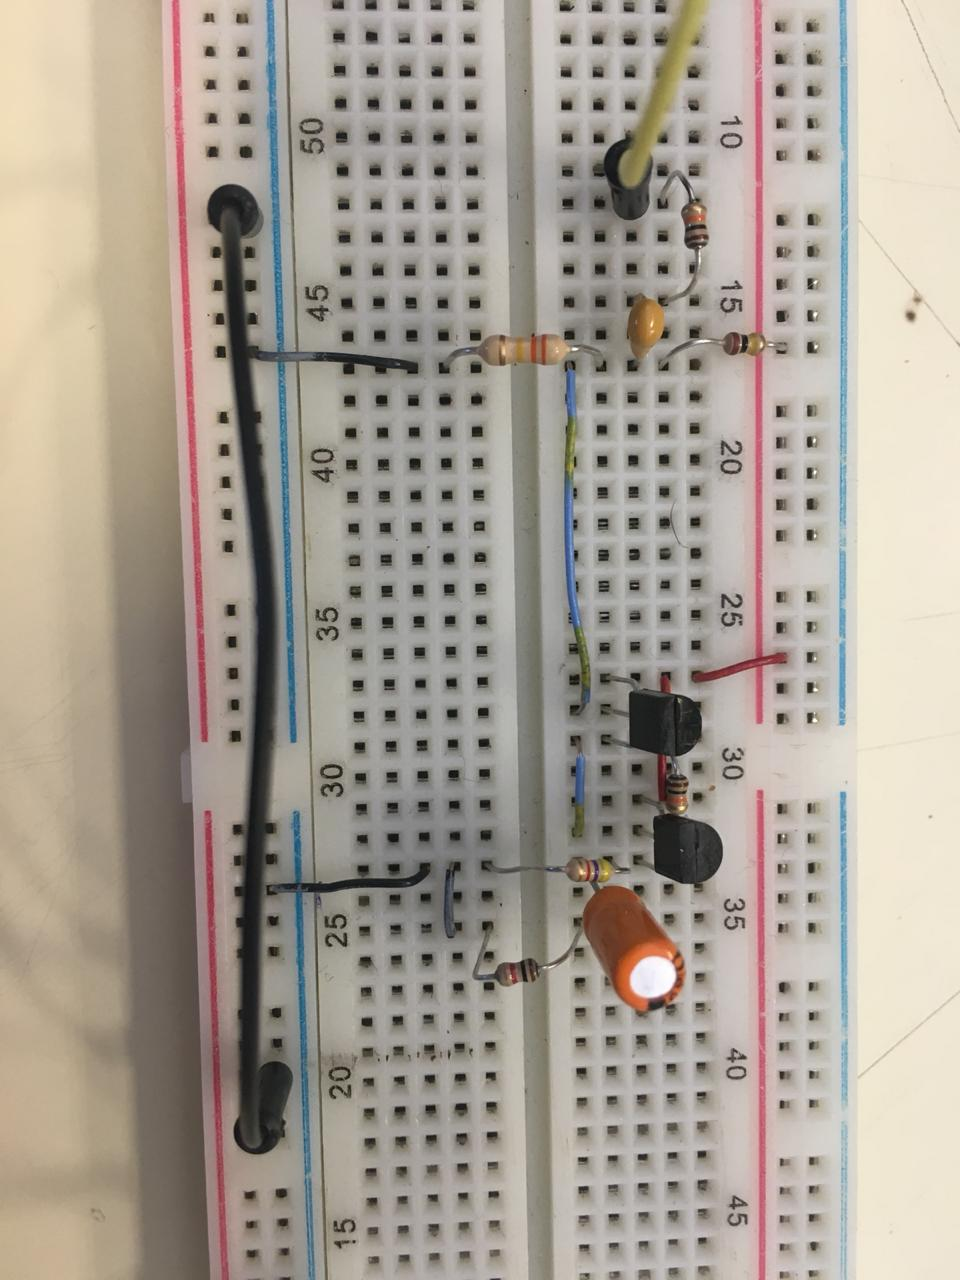
\includegraphics[scale=0.4]{./Imagenes/circuito_proto.jpeg} \\
			\caption{Circuito armado en protoboard.}
			\label{circ_proto}
		\end{figure}

\subsection{Polarización}
La comparación entre los valores de la polarización de los transistores se muestran en la Tabla\ref{tabla_polarizacion_comp}. Las diferencias en las $I_{CQ}$ se deben principalmente a las variaciones de $\beta$ con $I_{C}$, que fueron tenidas en consideración en los cálculos teóricos, pero de todas formas es distinto al real.

\todo{Insertar tabla polarización}

\subsection{Ganancias}
En primer lugar, se midió la ganancia de tensión del sistema. En la Figura \ref{fig_bode_avs} se muestra la constrastación de la medición, la simulación y la teoría. Como ningún cálculo teórico tiene en cuenta variaciones con la frecuencia, se toma un único valor para todas las frecuencias, y se ve que la aproximación para frecuencias medias es válida en el intervalo de frecuencias entre 400$Hz$ y 500$kHz$, donde la ganancia empieza a caer. La ganancia en la banda pasante simulada es de 0.87 veces y la medida llega hasta 0.9 veces, con lo que el cálculo teórico de 0.866 veces resulta muy cercano a la realidad.

		\begin{figure}[H]
			\centering
			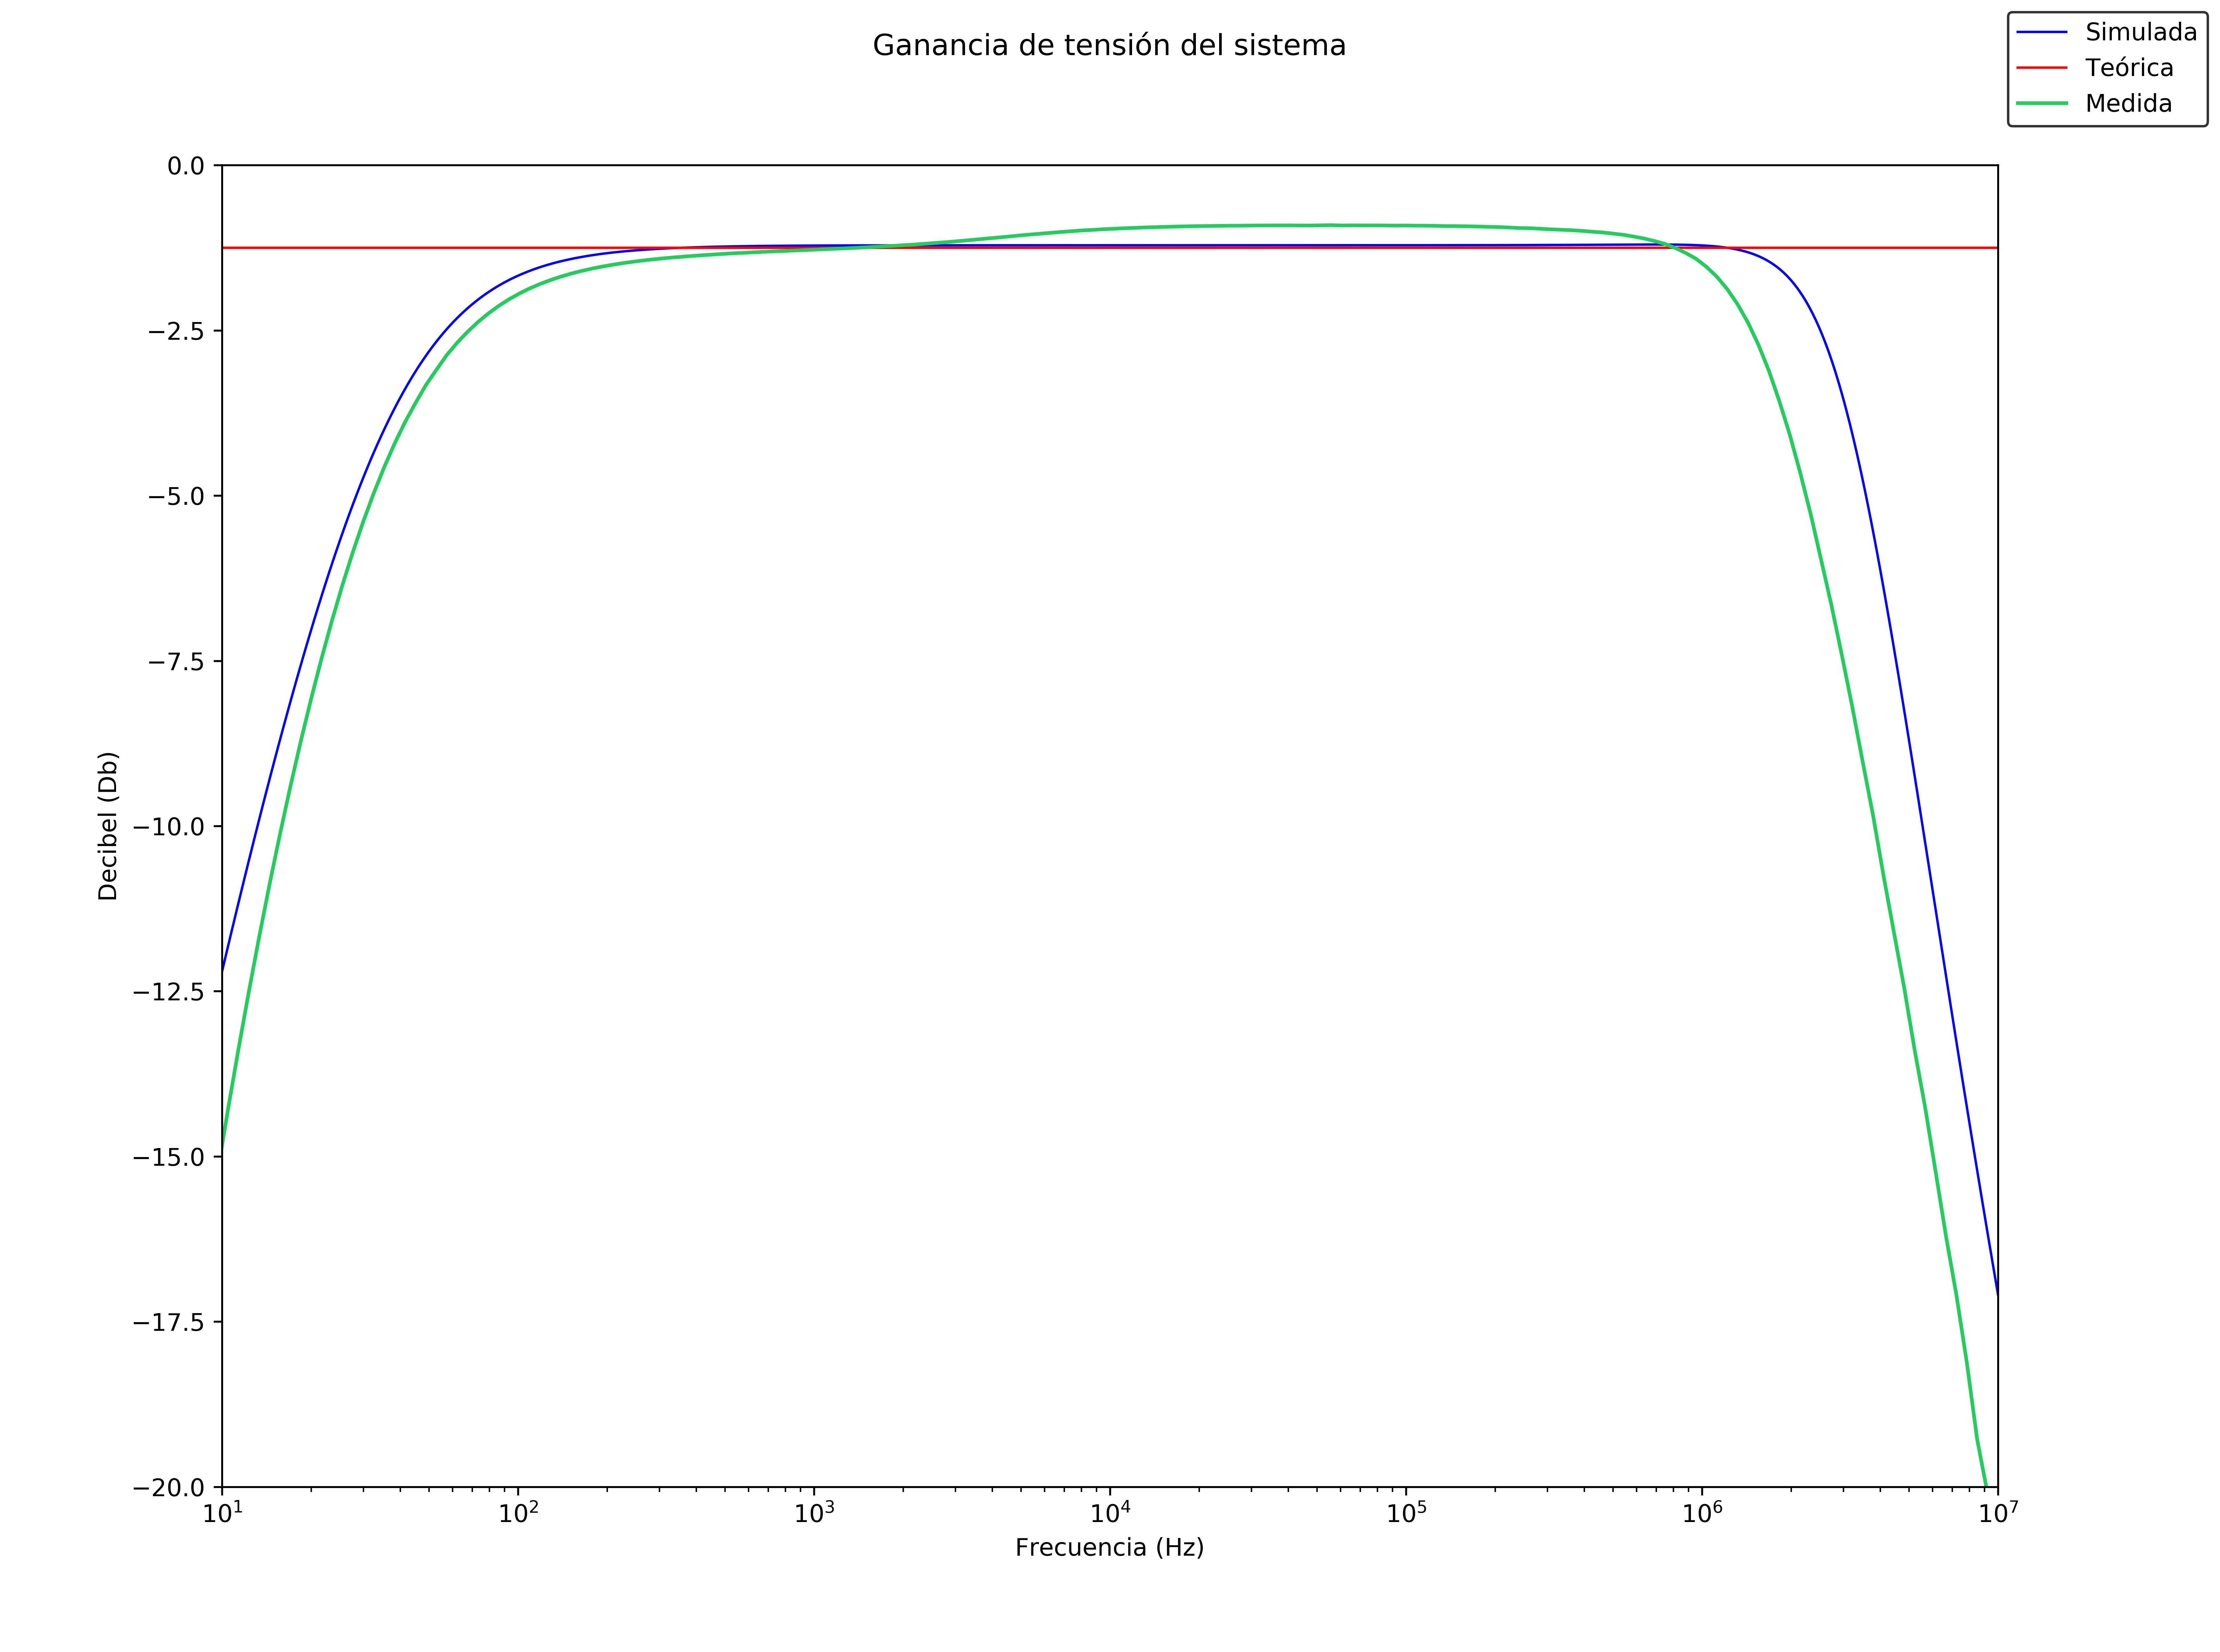
\includegraphics[scale=0.4]{./Imagenes/bode_Avs.png} \\
			\caption{Ganancia de tensión del sistema teórica, simulada y medida}
			\label{fig_bode_avs}
		\end{figure}

Luego se midió la ganancia de corriente del sistema. En la Figura \ref{fig_bode_ais} se puede observar la comparación entre teoría, simulación y práctica. En éste caso, es menor el intervalo de frecuencias en las que es válida la estimación teórica, y se presenta una diferencia entre simulación y medición en el punto en el que empieza a caer la ganancia. Éste efecto puede ser atribuible a las capacidades introducidas por el protobard. La ganancia en la banda pasante simulada y medida es de 37,5dB, es decir, 75 veces, mientras que la teórica es de 74 veces, con lo que el modelo nuevamente se verifica. 

\todo{Insertar valores más específicos de simulación y medición}

		\begin{figure}[H]
			\centering
			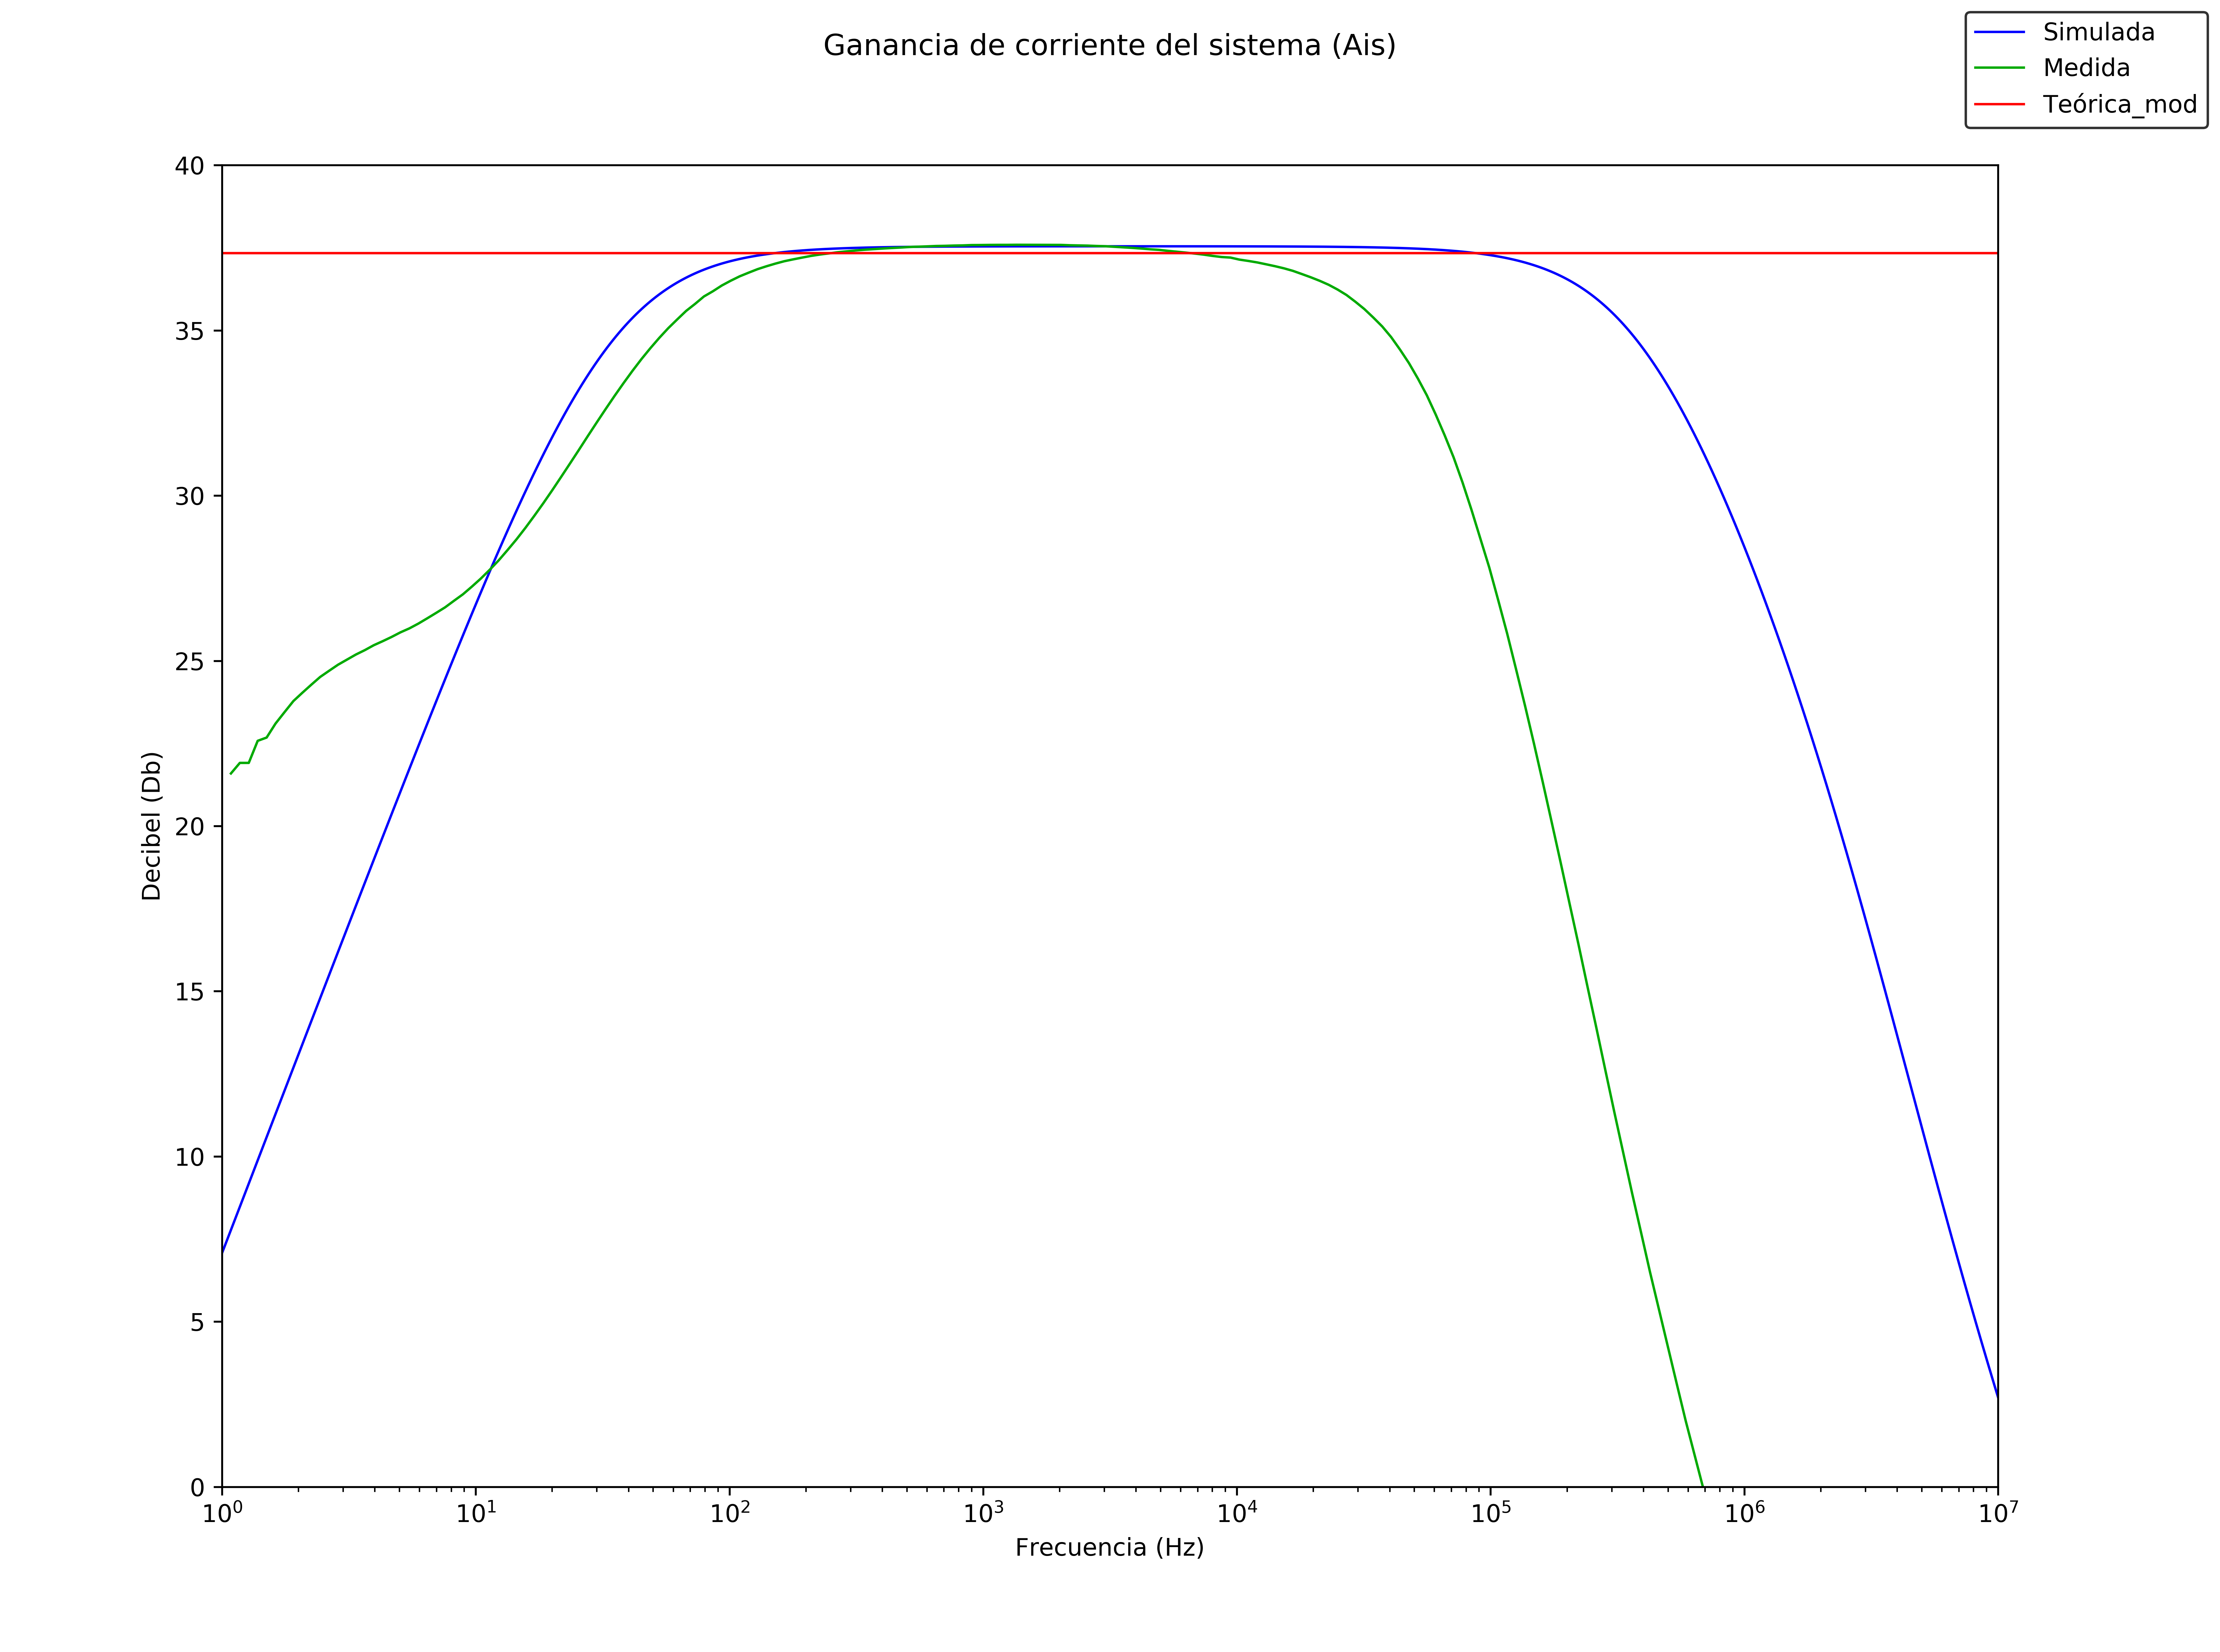
\includegraphics[scale=0.3]{./Imagenes/bode_Ais.png} \\
			\caption{Ganancia de corriente del sistema teórica, simulada y medida}
			\label{fig_bode_ais}
		\end{figure}

\subsection{Impedancias}
Con respecto a la impedancia de entrada, se muestra la contrastación entre teoría, simulación y medición en la Figura \ref{fig_bode_zin}, donde se puede apreciar que para frecuencias inferiores a 10$kHz$ las tres curvas son cercanas, siendo la impedancia de entrada medida a 200Hz $76,2k\Omega$, mientras que la simulada a la misma frecuencia es de $86,676k\Omega$ y la teórica es de $85k\Omega$. Nuevamente se observa que la medición no se corresponde con la medición a partir de 10$kHz$.

		\begin{figure}[H]
			\centering
			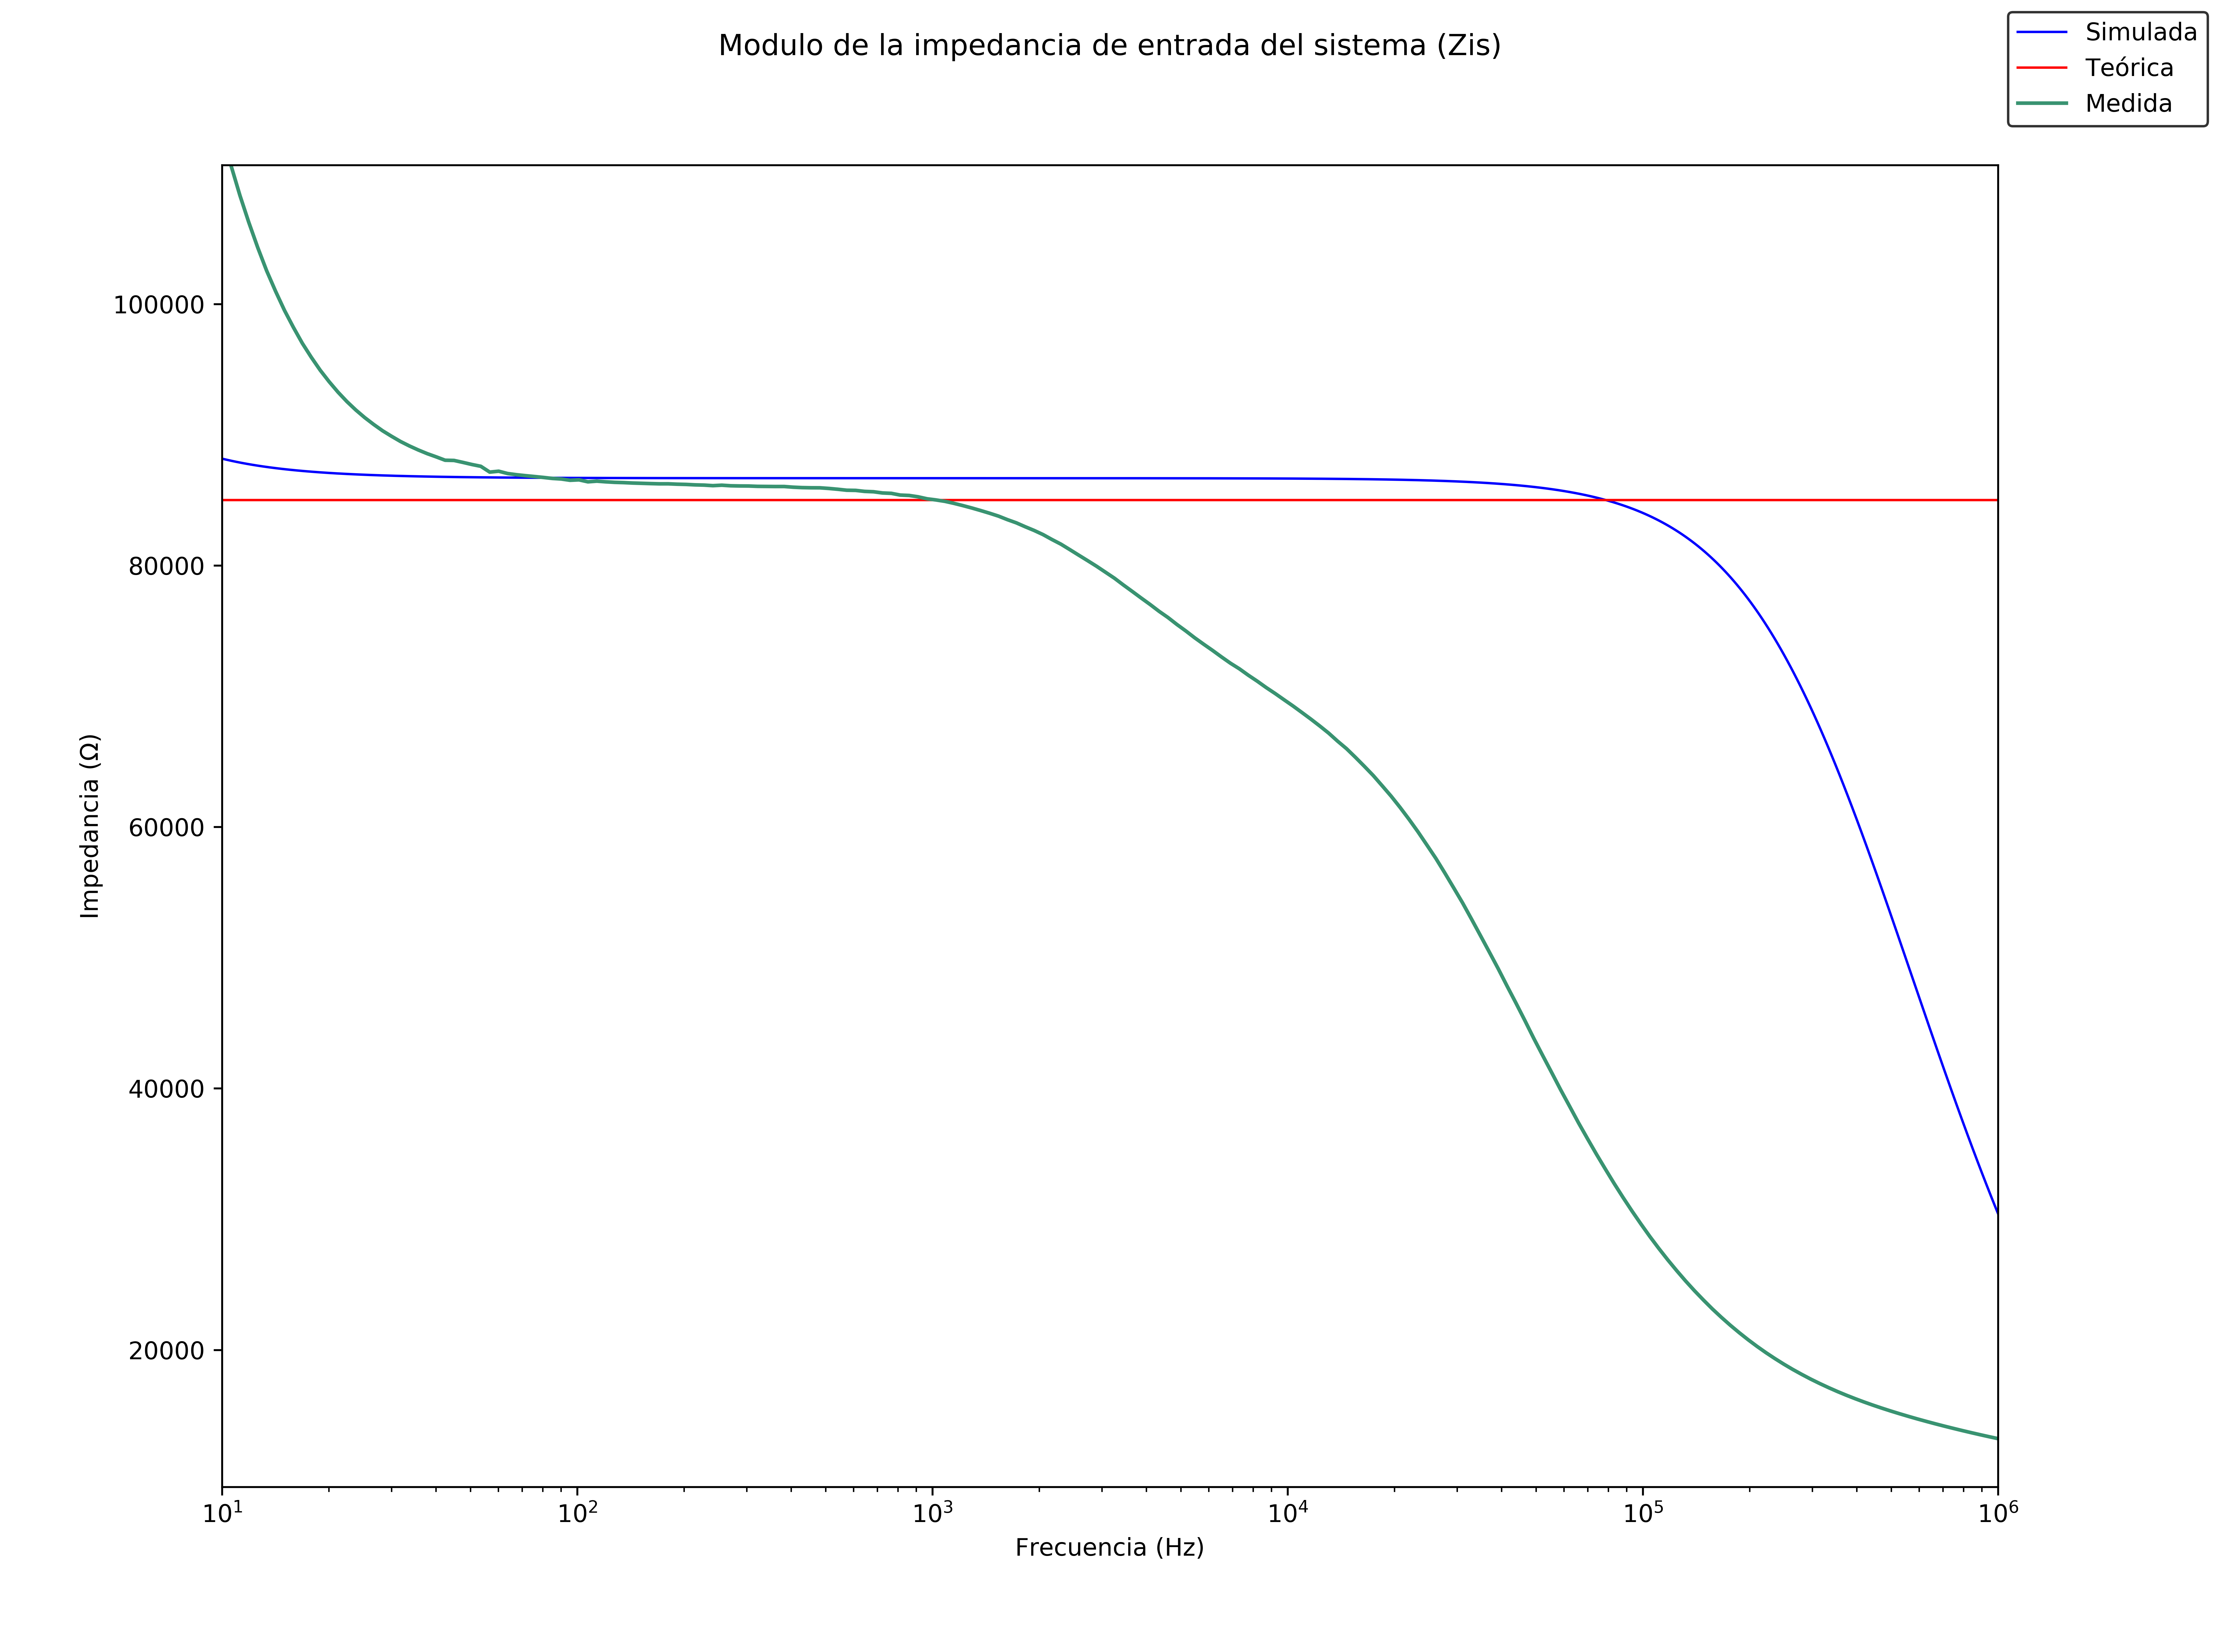
\includegraphics[scale=0.4]{./Imagenes/Modulo_zin.png} \\
			\caption{Impedancia de entrada del sistema teórica, simulada y medida.}
			\label{fig_bode_zin}
		\end{figure}

Para la impedancia de salida se muestra la contrastación entre teoría, simulación y práctica en la Figura \ref{fig_bode_zout}. Se observa que el sistema presenta una baja impedancia de salida, lo cual era esperado por tratarse de un colector común. 

\todo{Insertar valores}

		\begin{figure}[H]
			\centering
			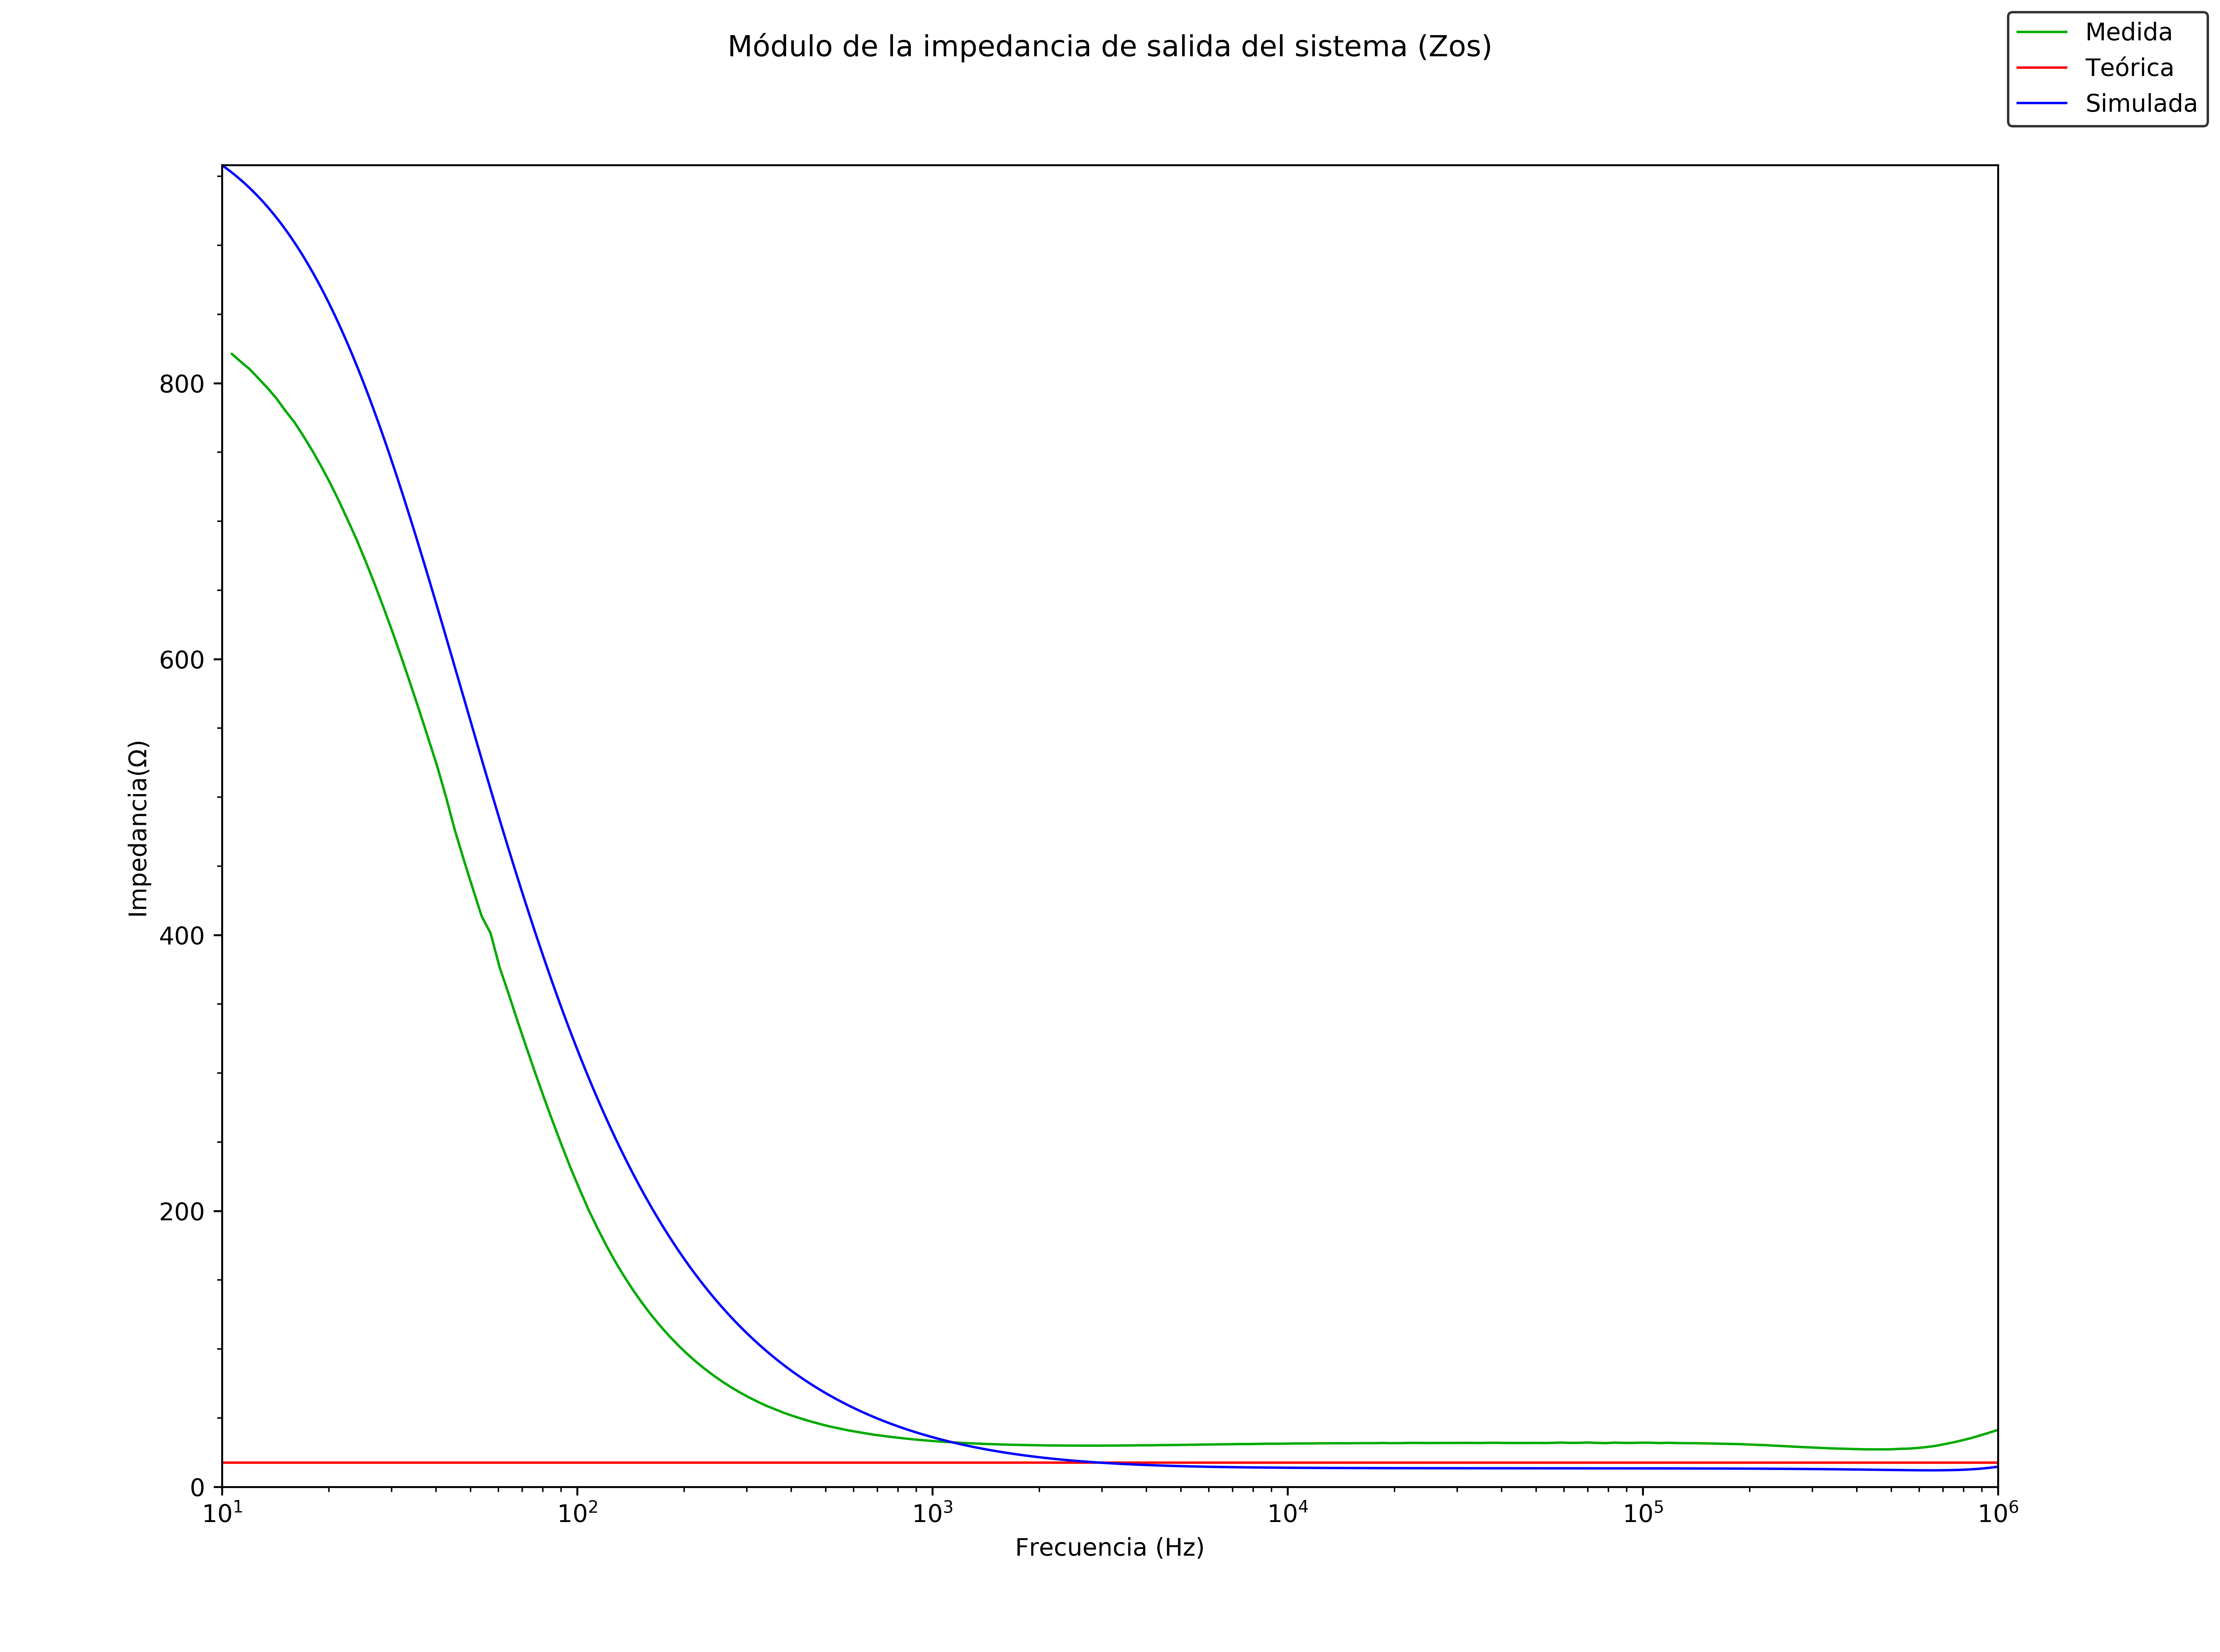
\includegraphics[scale=0.4]{./Imagenes/Modulo_zos.png} \\
			\caption{Impedancia de salida del sistema teórica, simulada y medida.}
			\label{fig_bode_zout}
		\end{figure}
 
\subsection{Resumen}

En la siguiente tabla se muestran los valores teóricos, simulados y medidos de las ganancias e impedancias para frecuencias medias. Se tomaron los valores para %___ kHz


\todo{Insertar tabla con los valores para frecuencias medias que den lindo, buscar en txt de simulaciones y csv de mediciones los que no estén puestos más arriba}